\documentclass[onecolumn,aps, pre,amsmath,amssymb,longbibliography,12pt]{revtex4-2}
\usepackage{graphicx}
% \usepackage{dcolumn}
\usepackage{bm}
\usepackage{amsfonts}
\usepackage{xcolor,tabu}
\usepackage{multirow}
\usepackage{amsthm}
\usepackage{textcomp}
\usepackage{tikz}
\usepackage[colorlinks=true,
            linkcolor=blue,
            urlcolor=blue,
            citecolor=blue]{hyperref}
\hypersetup{bookmarksopen=true}
\usepackage{xr}
\usepackage{float}

\begin{document}
\title{Droplet tracking}
\maketitle

We study the motion of liquid droplets immersed in bacterial suspensions, an active bath.
The most basic and foundamental observation on the motion is the trajectory.
To obtain trajectories from a large amount of images, we need to develop an automatic tracking software.
Figure~\ref{fig:sample-image}A shows a sample image from an experiment, and the goal is to find the inner droplet, as highlighted in Fig.~\ref{fig:sample-image}B.

\begin{figure}[h]
  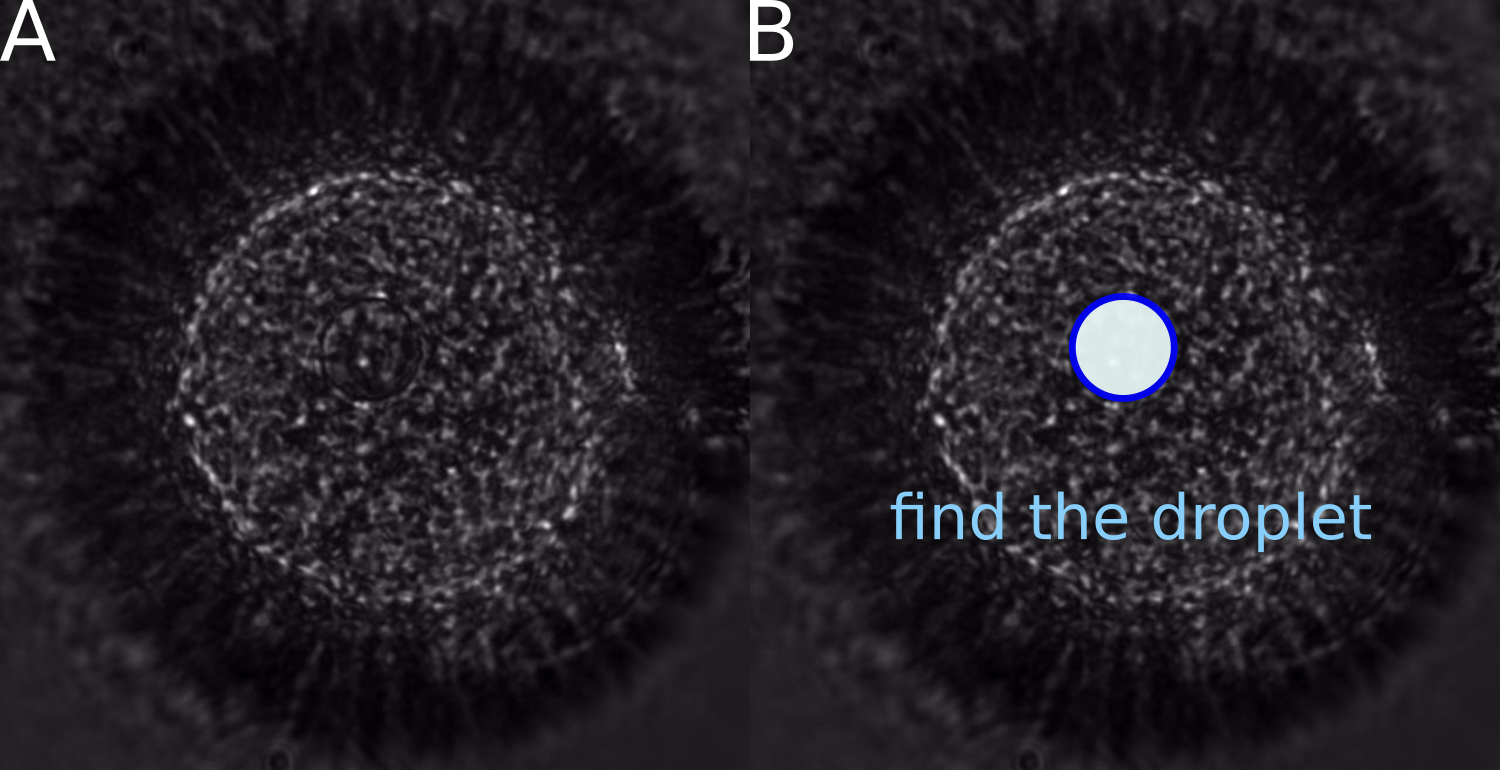
\includegraphics{sample-image.png}
  \caption{Sample image (A) and the goal of tracking software (B).}
  \label{fig:sample-image}
\end{figure}

\section{X-Y plane tracking}

I use corrTrack as the first attempt to find the inner droplet in the X-Y plane.
A description of corrTrack can be found in \href{https://github.com/ZLoverty/Python/tree/master/Tracking/corrTrack}{my Github repository}.
In this attempt, I used a binarized black circle as the mask (Fig.~\ref{fig:mask-and-result} inset), instead of a crop of the original image.
I did this because it is more general.
If the binarized mask works, it is very likely that a more specific mask, such as one cropped from the original image, will work.

\begin{figure}[h]
  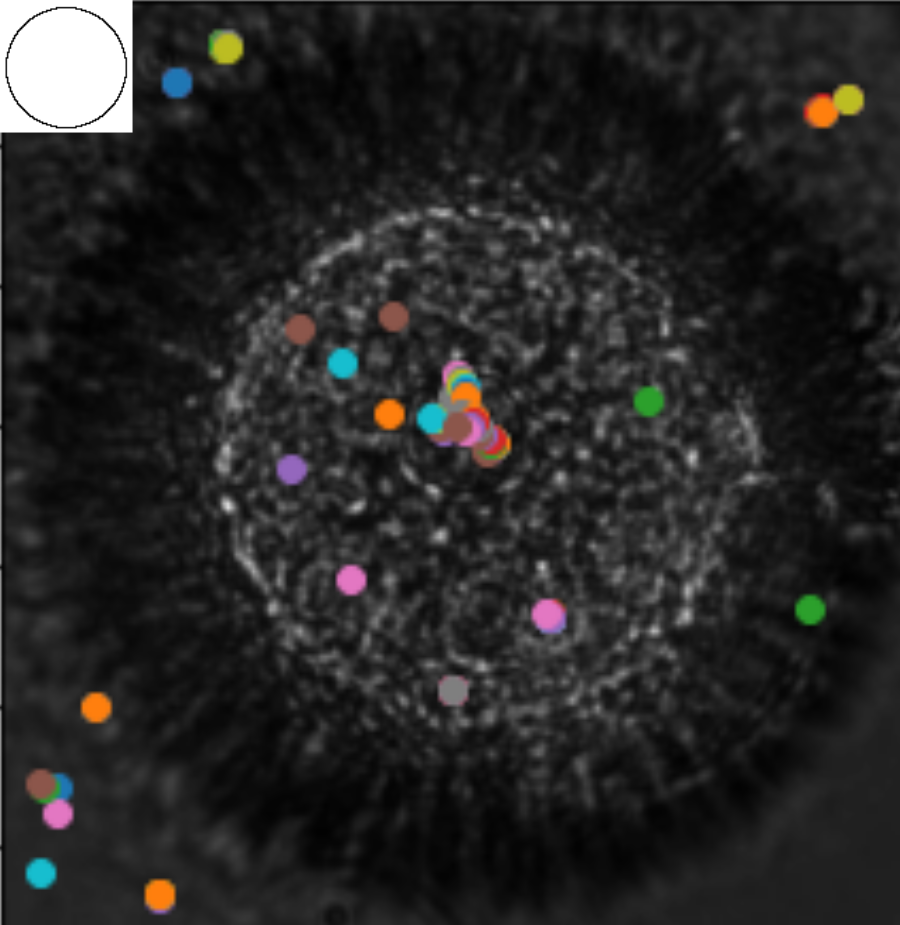
\includegraphics{mask-and-result}
  \caption{The mask used for corrTrack in the upper left corner.
  The result of the tracking is shown as colored circles, where different colors denote different times.}
  \label{fig:mask-and-result}
\end{figure}

The preliminary result of the tracking is shown in Fig.~\ref{fig:mask-and-result}.
While in some frames the software locates the inner droplet correctly, in most frames, however, the detection is erroneous.
Overall, the tracking does not work well.
To improve the quality of the tracking, we can
\begin{itemize}
  \item improve the image quality by adding fluorescent dyes to the inner droplets;
  \item use a specific mask, instead of a binarized mask;
  \item crop the image to avoid false tracking outside the droplets.
\end{itemize}

\textcolor{red}{These ideas should be tested and assessed in the future.}

\section{Z position}
As I wrote in the \textit{GOALS} note, the Z position of the inner droplet is crucial to understand the system.
On the one hand, we need the Z motions to interpret the dynamical properties, such as the diffusivity of the inner droplets we have measured in the X-Y plane;
on the other hand, it is a fingerprint behavior that should be compared with theoretical models.

We have proposed two ways to obtain Z positions: i) vertical scan and ii) tilted confocal.
Both methods have advantages and disadvantages.
Vertical scan can give X-Y position and Z position simultaneously.
But in each period of the scan, only one coordinate can be recorded.
Since the scan can not go as fast as the frame rate (typically 30 Hz), the resulting data would be sparce.
Confocal can record Z positions at a much higher rate, but simultaneously recording X-Y positions remains challenging.
\textcolor{red}{Test both options and assess.}

\subsection{Vertical scan}
The idea of vertical scan is illustrated in Fig.~\ref{fig:manual-scan}.
The inner droplet has slightly different lookings when it is in different positions relative to the focal plane.
When the droplet is below the focal plane, circular fringes can be seen around the droplets.
When the droplet is in the focal plane, the edge of the droplet is thin and sharp.
When the droplet is above the focal plane, the edge becomes thick and blurry.
(not sure if these images are from phase-contrast microscopy or bright field microscopy, need double-check)

\textcolor{red}{Compare 07132021 bright field images with Fig.~\ref{fig:manual-scan}. Need to make the extractImage notebook work properly.}

\begin{figure}
  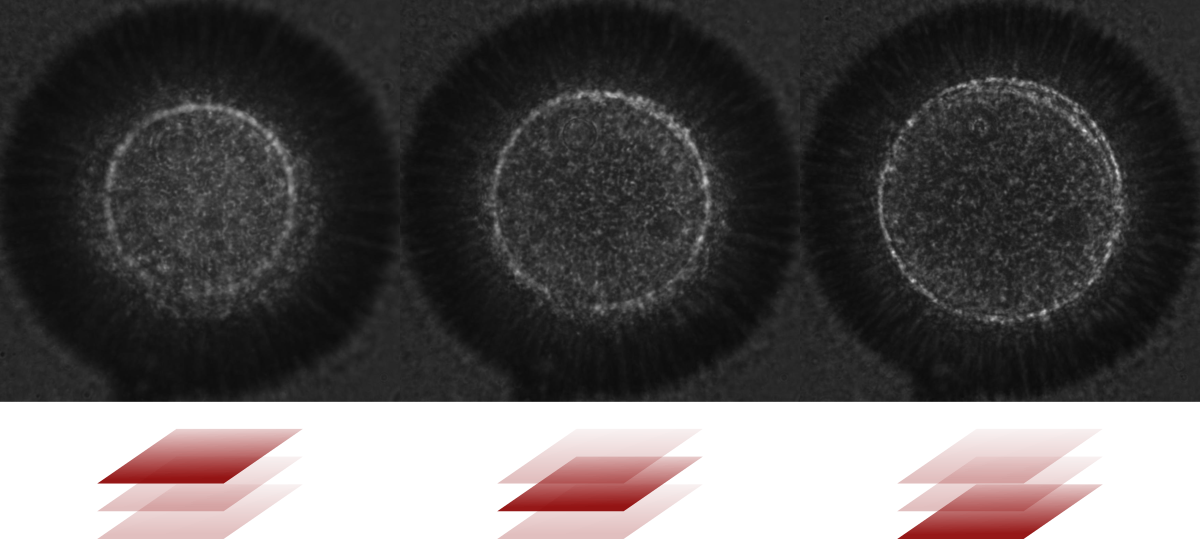
\includegraphics{manual-scan.png}
  \caption{Illustration of vertical scan.}
  \label{fig:manual-scan}
\end{figure}

\subsection{Tilted confocal}

\end{document}
